
%!TEX program = lualatex

\documentclass[a4paper,fleqn, headsepline, parskip=half, pagesize=dvips, twoside, final, openright, numbers=noenddot]{scrbook}

\usepackage{../../hft-thesis} % use same style as main document
\usepackage{../MyFigureStyle} % supplements for images




\begin{document}

\thispagestyle{empty}


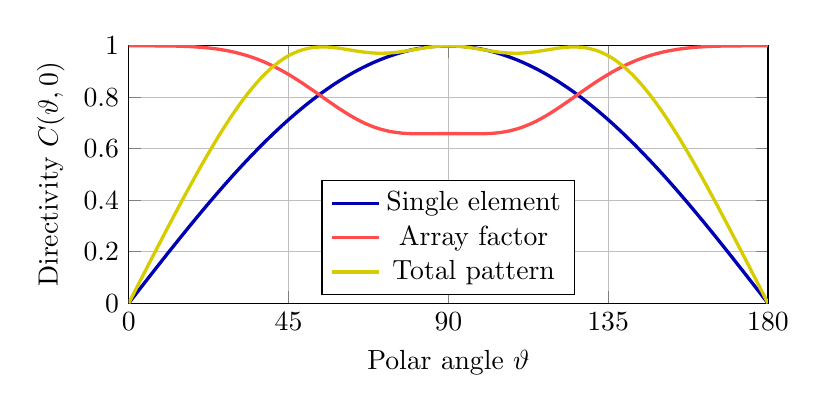
\begin{tikzpicture}
\begin{axis}[ 
width= 0.8\textwidth, 
height= 0.4\textwidth,
ymin=0,
ymax=1, 
xmin=0,
xmax=180,
xtick={0,45,90,135,180},
xlabel={Polar angle $\vartheta$},% \textrm{ in \SI{}{\degree}}$, % only for degree, symbol directly at number
xticklabel={\pgfmathprintnumber[precision=1]{\tick}\si{\degree}},
ylabel={Directivity $C(\vartheta,0)$},
grid=both,
samples=50,
domain=0:180,
%legend pos=south east, 
legend style={at={(0.5,0.03)},anchor=south}               %%%%%<<<<<----- change (.5,0) for anchor position, and anchor=south  means legend is above anchor
]
\addplot [blue!70!black,smooth,very thick]{sin(pi/10*sin(x)/pi*180)/sin(pi/10/pi*180)} ;
\addplot [red!70!white,smooth,very thick]{sqrt((1+2*0.263*cos(2.07/pi*180)*cos(180*cos(x)))^2+(2*0.263*sin(2.07/pi*180)*cos(180*cos(x)))^2) / sqrt((1+2*0.263*cos(2.07/pi*180)*cos(180*cos(0)))^2+(2*0.263*sin(2.07/pi*180)*cos(180*cos(0)))^2)} ;
\addplot [yellow!65!olive,smooth,very thick]{sin(pi/10*sin(x)/pi*180)/sin(pi/10/pi*180)* sqrt((1+2*0.263*cos(2.07/pi*180)*cos(180*cos(x)))^2+(2*0.263*sin(2.07/pi*180)*cos(180*cos(x)))^2) / sqrt((1+2*0.263*cos(2.07/pi*180)*cos(180*cos(90)))^2+(2*0.263*sin(2.07/pi*180)*cos(180*cos(90)))^2)} ;

\addlegendentry{Single element}
\addlegendentry{Array factor} 
\addlegendentry{Total pattern}
\end{axis}
\end{tikzpicture}  


\end{document}


